\chapter{まとめと今後の展望}
\section{結果}
本研究では、陽子線治療計画においてX線CTから得られる情報より陽子阻止能を求める際に生まれる不定性を解決するための方法として提案されている陽子線CTについて、新しいシステムを構築し検証を行った。\\
 世界的に研究がされているシリコンストリップ検出器を用いた陽子線CTは、構造が複雑であり測定時間が長いといった問題を抱えているが、本研究ではプラスチックシンチレータとCCDカメラを使用した簡単でコンパクトな実験装置を用いてCT画像を取得することに成功した。70MeV陽子線を用いたCT撮影では、直径$1mm$の穴が再構成画像上では$1.67mm$(FWHM)であった。この測定誤差は実際の陽子線治療におけるマージンよりも十分に小さいことから、実験の精度は問題のないレベルであると考えられる。また臨床応用を考えた際に必要となる200MeV陽子線においては、実寸で$89.30mm$の被写体がCT画像上では$89.79 \pm 0.22mm$であり、画像の鮮明さを表す被写体端部分でのESP(鮮鋭度)は6.5$^\circ$という結果から、鮮明かつ正確なCT画像を得ることに成功した。陽子阻止能に比例するWELの測定精度に関しては、70MeVにおいて5\%以下、200MeVにおいて11\%以下の精度で求めることが出来た。また再構成画像上で被写体の端内部が暗くなる多重クーロン散乱の影響は、特に密度差が大きくなる被写体と空気の境界面で顕著になるが、再構成画像から得た1次元プロファイル上でフーリエ変換をした後にフィルター処理を施すことで補正に成功した。

\section{今後の展望}
本研究では主に2つの課題が見つかった。1つ目が、シンチレータの劣化による精度悪化を防ぐこと、2つ目が被写体における多重クーロン散乱を補正すること、である。以下で詳しく見ていくこととする。

\subsection{シンチレータの劣化による精度悪化を防ぐ}
70MeV陽子線を用いたCT撮影では、30nAという高レート照射のためシンチレータが劣化しWEL測定の精度が落ちた。したがって、発光量の多いシンチレータを用いて低レートで測定を行うことが望まれる。またシンチレータ内での多重クーロン散乱の影響を無視出来るよう、シンチレータが十分に薄いことも条件となる。これより本研究に適すると考えられるのが、X線CTで用いられる増感紙である。医療におけるX線検査は、患者の被爆を最小限にしながら診断に適当な画質を確保することが望まれる。高画質な画像を得るためには十分な発光量が必要であり、低線量照射においてX線フィルムの乳剤の感度を増進させるために、増感紙を乳剤に接するように置くことがある。増感紙は高い原子番号を持つ光放出蛍光剤からなり、これによりX線に対するフィルムの感度は10倍程度増加する。\\
 陽子線に対する増感紙の感度を調べるために投影画像を取得した。用いた増感紙は富士フイルム株式会社の富士医療用増感紙HR-16であり、ポリエチレンテレフタレートでできた支持体に$Gd_{2}O_{2}S:Tb$(密度$7.34[g/cm^{3}]$)などの蛍光体を塗布したもので、厚みは$1mm$程度である。高さ7cmのアクリル円柱に対して第---章と同様の条件(200MeV、10nA、照射時間0.5秒)で取得した投影画像が図\ref{GOS}である。被写体がない部分(a)を基準としたとき、被写体部分(b)の発光量比は1.080であった。プラスチックシンチレータにおいては1.065倍であり、増感紙を用いたことによりコントラストがはっきりすることが分かる。これは主に、プラスチックシンチレータの線量と発光量の関係が非線形であることが原因だと考えられる。シンチレータの厚みが50分の1になっても発光量は同等以上であり、またシンチレータを薄くすることで、シンチレータ内での散乱の影響が小さくなるだけでなく、被写体の散乱により曲げられた陽子線におり発光が領域が幅を持つという影響も少なくなるという利点があり、今後増感紙を用いた陽子線CTに挑戦したいと考える。
\begin{figure}[H]
\centering
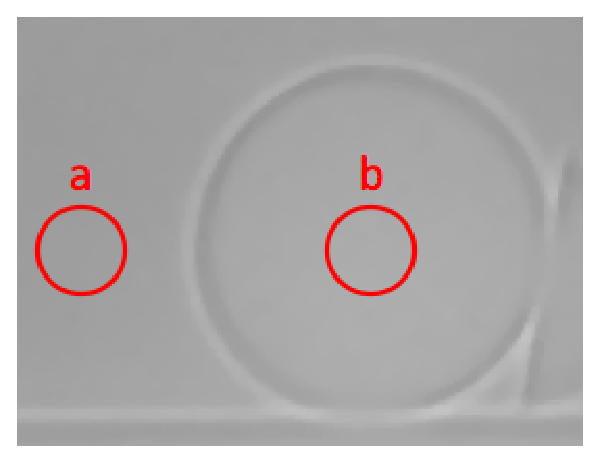
\includegraphics[width=7cm]{eps/NextWork/GOS.eps}
\caption{増感紙を用いた陽子線投影画像}
\label{GOS}
\end{figure}

\subsection{被写体における多重クーロン散乱を補正する}
第---章において、再構成画像の1次元プロファイルにおいて、多重クーロン散乱の補正に成功したことを述べた。2次元に拡張するにあたり、2つの方法を考えている。\\
 1つ目は、1次元での補正同様に再構成画像を2次元フーリエ変換し、散乱がない場合の変換画像と比較して、散乱の影響による余分な部分をフィルター補正する方法である。または、サイノグラムが原画像の1次元フーリエ変換と同等であることから、再構成過程でサイノグラムを1次元フーリエ変換したデータにフィルター補正をする方法もある。これは、投影データが$\theta$について連続的に取得出来ないことから、逆フーリエ変換において極座標から直交座標に再配置する際に高周波成分ほどデータが粗になることを補間するランプフィルターに、さらに多重クーロン散乱の補正項を追加することを意味する。しかし、これはシミュレーションベースの研究になってしまうことから、2つ目の方法として被写体-シンチレータ間の距離を変えた2枚の取得画像の差をとることを考えている。距離に対して散乱の影響が規則的に表されれば、取得画像から散乱を除くことも可能となる。

%\end{document}